\documentclass[aspectratio=169,11pt,t]{beamer}
% ============================================================
%  ksa-cs-v2: ksa-cs-lecture-template.tex 스타일 + 한글, v2 덱(16:9)용.
%    - 짙은 네이비 헤드라인 (섹션 이름 + 프레임마다 점)
%    - 꽉 찬 파란 제목 막대, 둥근 그림자 블록
%    - 한글: Noto Sans CJK KR (fontspec)
%  사용:
%    \documentclass[aspectratio=169,11pt,t]{beamer}
%    \input{<..>/theme/ksa-cs-v2.tex}
%  ksa-theme.tex 의 매크로(\kb \kq, ksablue/ksared 등)도 같은 이름으로 둔다
%  -> v2 덱 본문을 거의 그대로 옮길 수 있다.
% ============================================================

\usepackage{fontspec}
\usepackage{amsmath,amssymb}
\usepackage{tikz}
\usepackage{listings}
\usepackage{graphicx}
\usepackage{booktabs}
\usepackage{varwidth}
% enumitem 은 넣지 않는다 (beamer 글머리표가 사라진다)

\defaultfontfeatures{Ligatures=TeX}
\setmainfont{Noto Sans CJK KR}
\setsansfont{Noto Sans CJK KR}
\setmonofont{Noto Sans Mono CJK KR}[Scale=0.92]
\usefonttheme{professionalfonts}

% ---------- 기본 틀 ----------
\usetheme{default}
\useinnertheme[shadow=true]{rounded}
\setbeamertemplate{navigation symbols}{}
\setbeamersize{text margin left=1em,text margin right=1em}

% ---------- 색 (템플릿 원본 값) ----------
\definecolor{navydark}{HTML}{191959}
\definecolor{navydim}{HTML}{8888B0}
\definecolor{navytitle}{HTML}{262686}
\definecolor{navyblue}{HTML}{3333B2}
\definecolor{blockbodybg}{HTML}{E9E9F3}
\definecolor{examplegreen}{HTML}{006000}
\definecolor{examplebg}{HTML}{E5EFE5}
\definecolor{alertred}{HTML}{BF0000}
\definecolor{alertbg}{HTML}{F9E5E5}
% ksa-theme.tex 와 같은 이름 (본문 호환)
\colorlet{ksablue}{navytitle}
\colorlet{ksabluedk}{navydark}
\definecolor{ksagold}{HTML}{D6CBB1}
\definecolor{ksagolddk}{HTML}{A9976B}
\colorlet{ksared}{alertred}
\definecolor{ksagray}{HTML}{5B5B5B}

\setbeamercolor{structure}{fg=navyblue}
\setbeamercolor{alerted text}{fg=alertred}
\setbeamercolor{frametitle}{bg=navytitle,fg=white}
\setbeamercolor{title}{fg=white,bg=navytitle}
\setbeamercolor{block title}{bg=navytitle,fg=white}
\setbeamercolor{block body}{bg=blockbodybg,fg=black}
\setbeamercolor{block title example}{bg=examplegreen,fg=white}
\setbeamercolor{block body example}{bg=examplebg,fg=black}
\setbeamercolor{block title alerted}{bg=alertred,fg=white}
\setbeamercolor{block body alerted}{bg=alertbg,fg=black}
\setbeamercolor{item}{fg=navyblue}
\setbeamertemplate{itemize item}[circle]
\setbeamertemplate{itemize subitem}[triangle]

% ---------- 헤드라인: miniframes (섹션 이름 + 점) ----------
\useoutertheme[subsection=false]{miniframes}
\setbeamerfont{section in head/foot}{size=\tiny}
\setbeamercolor{section in head/foot}{bg=navydark,fg=white}
\setbeamercolor{mini frame}{fg=white}
\setbeamertemplate{mini frames}[circle]

% ---------- 제목 막대: 폭 꽉 채움, 두 줄까지 ----------
\setbeamerfont{frametitle}{size=\normalsize,series=\bfseries}
\setbeamertemplate{frametitle}{%
  \nointerlineskip
  \begin{beamercolorbox}[wd=\paperwidth,ht=2.7ex,dp=1.1ex,leftskip=.3cm,rightskip=.3cm]{frametitle}%
    \usebeamerfont{frametitle}\insertframetitle
  \end{beamercolorbox}}

% ---------- 쪽 번호: 오른쪽 아래 ----------
\setbeamertemplate{footline}{%
  \hfill
  {\color{navydim}\scriptsize\insertframenumber\,/\,\inserttotalframenumber}%
  \hspace{3mm}\vspace{2mm}%
}

% ---------- 표지: 템플릿처럼 헤드라인은 그대로, 가운데 둥근 그림자 상자에 제목 한 줄 ----------
% 덱에서:  {\setbeamertemplate{footline}{}\begin{frame}[c,noframenumbering]\titlepage\end{frame}}
\setbeamercolor{title}{fg=white,bg=navyblue}
\makeatletter
\setbeamertemplate{title page}{%
  \vfill
  \centering
  \begin{minipage}{0.84\paperwidth}
  \begin{beamercolorbox}[wd=\linewidth,sep=7pt,center,rounded=true,shadow=true]{title}
    {\usebeamerfont{title}\inserttitle\par}%
    \ifx\insertsubtitle\@empty\else\vskip0.4em{\usebeamerfont{subtitle}\insertsubtitle\par}\fi
  \end{beamercolorbox}
  \end{minipage}\par\vskip1.6em
  {\usebeamerfont{author}\color{navytitle}\insertauthor\par}\vskip0.3em
  {\usebeamerfont{institute}\color{ksagray}\insertinstitute\par}
  \vfill
}
\makeatother
\setbeamerfont{title}{series=\bfseries,size=\Large}
\setbeamerfont{subtitle}{size=\normalsize}
\setbeamerfont{author}{size=\normalsize}
\setbeamerfont{institute}{size=\small}

% ksa-theme 호환: 덱이 \renewcommand{\ksacredit}{..} 를 해도 되게 (꼬리말에는 안 쓴다)
\newcommand{\ksacredit}{}

% ---------- 강조 ----------
\newcommand{\hl}[1]{\textcolor{alertred}{#1}}
\newcommand{\hlb}[1]{\textcolor{navyblue}{#1}}
\newcommand{\kb}[1]{\textbf{\color{ksablue}#1}}
\newcommand{\kq}[1]{\textbf{\color{ksared}#1}}

% ---------- 파이썬 코드 (템플릿과 같은 색) ----------
\definecolor{codekw}{HTML}{0033B3}
\definecolor{codebuiltin}{HTML}{BF0000}
\definecolor{codestr}{HTML}{067D17}
\definecolor{codecomment}{HTML}{8C8C8C}
\definecolor{codenum}{HTML}{1750EB}
\lstdefinestyle{py}{
  language=Python, basicstyle=\ttfamily\scriptsize,
  keywordstyle=\color{codekw}\bfseries, stringstyle=\color{codestr},
  commentstyle=\color{codecomment}\itshape, numberstyle=\color{codenum},
  emph={print,len,range,sum,input,int,str,float,list,dict,append,remove,sorted,abs,min,max},
  emphstyle=\color{codebuiltin}, showstringspaces=false, keepspaces=true,
  columns=fixed, basewidth=0.52em, aboveskip=1mm, belowskip=1mm, xleftmargin=2mm,
  breaklines=true
}
\lstset{style=py}

% 원본 덱 (ksa-theme): slides/v2/ml1/week13/gcn/ -- 그림은 거기 figs/ 를 그대로 쓴다
\setbeamerfont{author}{size=\normalsize}
\setbeamerfont{institute}{size=\small}
\graphicspath{{../../../v2/ml1/week13/gcn/figs/}{../../../assets/}}
\makeatletter
\newcommand{\markpage}[1]{\protected@write\@auxout{}{\string\newlabel{#1}{{\the\c@framenumber}{}}}\hypertarget{#1}{}}
\newcommand{\pref}[1]{\hyperlink{#1}{\textcolor{ksagolddk}{(p.\ref{#1})}}}
\makeatother

\renewcommand{\ksacredit}{Machine Learning and Deep Learning \,\textperiodcentered\, GCN}
\title{GCN 그래프 신경망 (Graph Convolutional Network)}
\subtitle{나와 친구들의 평균으로 층을 쌓는다}
\author{Machine Learning and Deep Learning}
\institute{한국과학영재학교 (KSA)}
\date{}
\begin{document}
{\setbeamertemplate{footline}{}\begin{frame}[c,noframenumbering]\titlepage\end{frame}}


\section{질문}
% --- 오늘의 질문
\begin{frame}{오늘의 질문: 나머지 32명은 어느 편일까?}
\vfill
\begin{columns}[c]
\column{0.5\linewidth}\centering
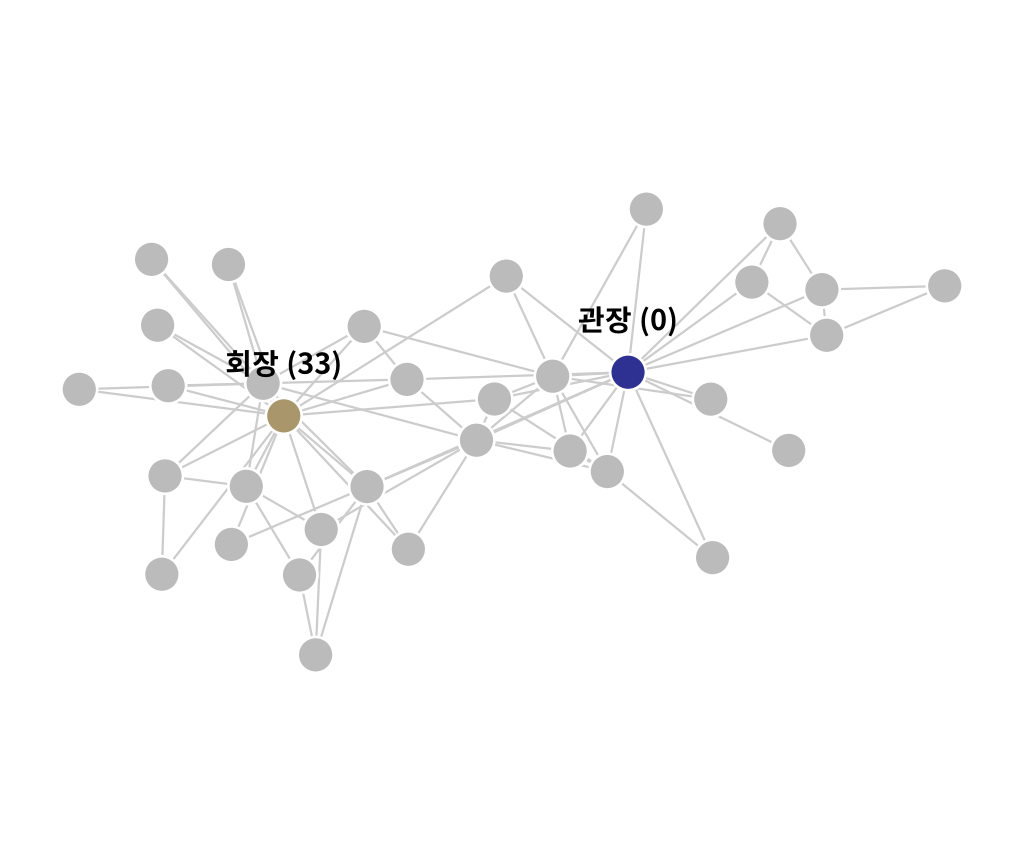
\includegraphics[width=\linewidth]{gc_question.png}
\column{0.48\linewidth}
{\large 1977년 미국 대학의 가라테 동아리}\\[0.4em]
{\large \kb{34}명, 친구 관계 \kb{78}개 (Zachary 1977)}\\[0.4em]
{\large 관장과 회장이 다투다 동아리가 \textbf{둘로 쪼개졌다}}\\[1em]
{\large 편이 알려진 건 \textcolor{ksablue}{관장} · \textcolor{ksagolddk}{회장} \kq{2명}뿐}\\[0.4em]
{\large 친구 관계만 보고 나머지 32명을 맞힐 수 있을까?}
\end{columns}
\vfill
\note{1977년 미국의 한 대학 가라테 동아리입니다. 34명이 있었고, 동아리 밖에서도 어울리는 친구 관계가 78개 있었습니다. 인류학자 재커리가 기록했는데, 관장과 회장이 수업료 문제로 다투다 동아리가 둘로 쪼개졌습니다. 우리가 아는 건 관장과 회장 두 사람의 편뿐입니다. 친구 관계만 보고 나머지 32명이 어느 편으로 갔는지 맞힐 수 있을까요? 오늘은 이런 연결된 데이터를 위한 신경망, GCN을 배웁니다.}
\end{frame}

\section{그래프}
% --- 그래프
\begin{frame}{그래프: 점과 선}
\vfill
\centering
\renewcommand{\arraystretch}{1.5}
{\large\begin{tabular}{lll}
노드 (점) & 사람 \quad 원자 \quad 교차로 \quad 논문 & 특징 벡터 $\mathbf{x}_i$\\
엣지 (선) & 친구 \quad 결합 \quad 도로 \quad 인용 & 인접 행렬 $A_{ij} = 1$ (이어짐), $0$ (아님)
\end{tabular}}\vskip0.8em
{\large 표 데이터 · 이미지 · 문장과 다른 점}\\[0.3em]
{\large 이웃 수가 \textbf{제각각} (가라테: 1명 $\sim$ 17명)}\\[0.2em]{\large 정해진 \textbf{순서}가 없다 (누가 1번이든 같은 그래프)}\\[0.6em]
{\small 이미지 = 모든 픽셀이 이웃 8개인 격자 그래프 \quad 문장 = 앞뒤로만 이어진 줄 그래프}
\vfill
\note{그래프는 점과 선입니다. 점을 노드, 선을 엣지라고 합니다. 가라테 동아리에서는 사람이 노드, 친구 관계가 엣지이고, 분자에서는 원자와 결합, 도로망에서는 교차로와 도로, 논문에서는 논문과 인용입니다. 노드마다 특징 벡터 x가 있고, 연결은 인접 행렬 A로 씁니다. 이어져 있으면 1, 아니면 0입니다. 지금까지 다룬 데이터와 다른 점은, 이웃 수가 제각각이라는 것, 가라테에서는 1명부터 17명까지입니다. 그리고 정해진 순서가 없습니다. 사실 이미지는 모든 픽셀이 이웃 8개인 격자 그래프이고, 문장은 앞뒤로만 이어진 줄 그래프입니다.}
\end{frame}

\section{GCN}
% --- 아이디어
\begin{frame}{GCN: 새 정보 = 나와 친구들의 평균}
\markpage{idea}
\vfill
\centering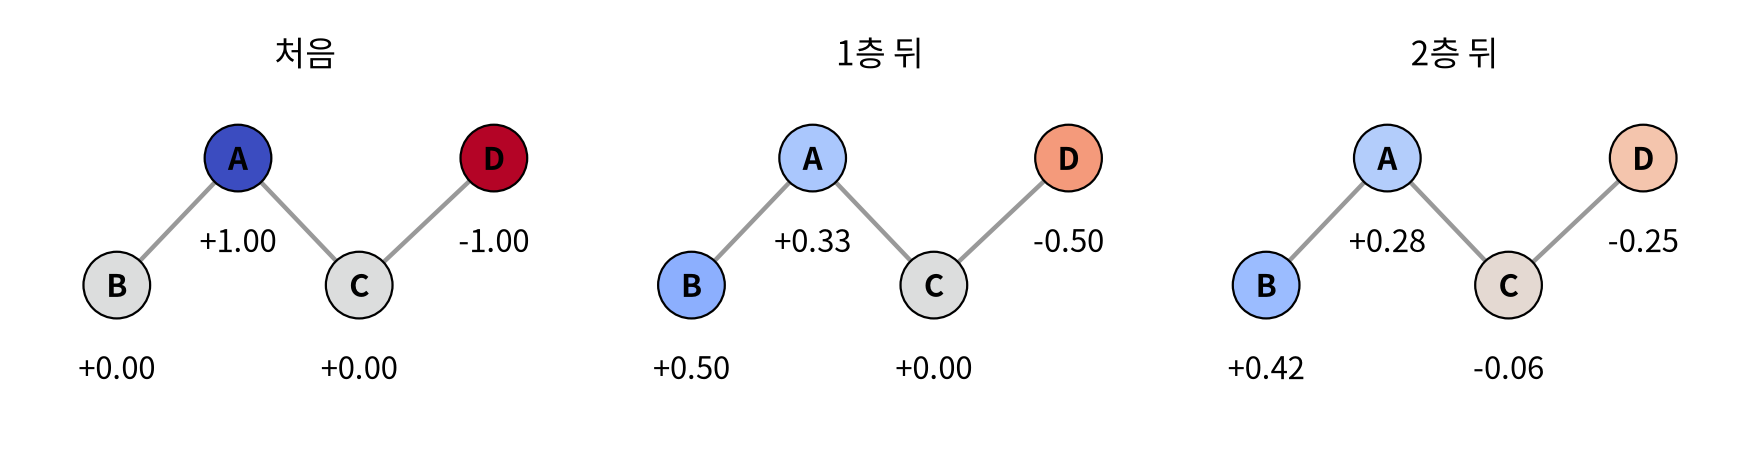
\includegraphics[width=0.8\linewidth]{gc_hand.png}\par\vskip0.2em
{\large A = \textcolor{ksablue}{$+1$}, D = \textcolor{ksared}{$-1$} \quad 1층: \ B $= \dfrac{0 + 1}{2} = 0.5$, \ C $= \dfrac{0 + 1 - 1}{3} = 0$}\\[0.2em]
{\large 2층을 쌓으면 \kb{친구의 친구}까지 정보가 닿는다 \quad (C $= -0.06$: D 쪽으로 기운다)}
\vfill
\note{GCN의 아이디어는 간단합니다. 각 사람의 정보를 나와 친구들의 평균으로 바꿉니다. 네 명짜리 예로 해 봅시다. A는 관장 편이라 플러스 1, D는 회장 편이라 마이너스 1, B와 C는 모르니 0입니다. 한 층 지나면, B는 자기 0과 친구 A의 1을 평균 내 0.5, C는 자기 0, A의 1, D의 마이너스 1을 평균 내 0입니다. A는 0.33, D는 마이너스 0.5가 됩니다. 이걸 모두에게 동시에 하면 한 층입니다. 한 층 더 쌓으면 친구의 친구까지 정보가 닿아서, C가 마이너스 0.06으로 D 쪽으로 조금 기웁니다.}
\end{frame}

% --- 식
\begin{frame}{식으로: Kipf \& Welling (2017)}
\markpage{formula}
\vfill
\centering
{\LARGE\[ H^{(l+1)} = \sigma\!\left( \hat{A}\, H^{(l)}\, W^{(l)} \right), \qquad \hat{A} = D^{-1/2} (A + I)\, D^{-1/2} \]}\vskip0.4em
\renewcommand{\arraystretch}{1.5}
{\large\begin{tabular}{ll}
$A + I$ & 친구 + \textbf{나 자신} (자기 고리)\\
$D^{-1/2} \cdots D^{-1/2}$ & 친구 수로 나눈다: $\hat{A}_{ij} = 1 / \sqrt{d_i d_j}$ \quad ``평균'' 과 비슷\\
$W^{(l)}$ & 모든 노드가 \textbf{같은} 가중치를 쓴다 (CNN 의 필터처럼)\\
$\sigma$ & ReLU, 마지막 층은 softmax
\end{tabular}}\\[0.4em]
{\small 손 계산의 A–B: $d_A = 3$, $d_B = 2$ (자기 포함) $\to$ $\hat{A}_{AB} = 1 / \sqrt{6} = 0.41$ \quad (평균이면 $1/3$ 또는 $1/2$)}
\vfill
\note{식으로 쓰면 Kipf와 Welling이 2017년에 낸 GCN입니다. 다음 층의 특징 H는 A 햇 곱하기 H 곱하기 W에 활성화 함수를 씌운 것입니다. A 햇은 인접 행렬에 단위 행렬을 더해 나 자신도 포함하고, 양쪽에서 친구 수의 제곱근으로 나눈 행렬입니다. 그래서 A 햇의 ij 칸은 1 나누기 루트 d_i d_j, 평균과 비슷하지만 친구가 많은 사람의 영향은 조금 줄입니다. 손 계산의 A와 B 사이는 1 나누기 루트 6, 0.41입니다. W는 모든 노드가 같은 가중치를 씁니다. CNN에서 모든 위치가 같은 필터를 쓴 것과 같습니다.}
\end{frame}

% --- CNN 과 비교
\begin{frame}{왜 ``합성곱'' 인가}
\vfill
\centering
\renewcommand{\arraystretch}{1.6}
{\large\begin{tabular}{lll}
 & CNN (9주차) & GCN\\\hline
모으는 대상 & 이웃 픽셀 3 × 3 & 이웃 노드 (수가 제각각)\\
가중치 & 모든 위치가 같은 필터 & 모든 노드가 같은 $W$\\
층을 쌓으면 & 보는 범위가 넓어진다 & 몇 걸음 떨어진 노드까지\\
이웃의 순서 & 위 · 아래 · 왼쪽 $\cdots$ 구분 & 구분 없음 (더하기라 순서 상관없음)
\end{tabular}}\vskip0.6em
{\large 이웃을 \textbf{같은 가중치로} 모아 층을 쌓는다 \quad $\to$ 그래프 합성곱}
\vfill
\note{왜 그래프 합성곱이라고 부를까요? 9주차 CNN은 이웃 픽셀 3 곱하기 3을 모으고, 모든 위치가 같은 필터를 썼습니다. 층을 쌓으면 보는 범위가 넓어졌죠. GCN도 이웃 노드를 모으고, 모든 노드가 같은 가중치를 쓰며, 층을 쌓으면 몇 걸음 떨어진 노드까지 봅니다. 다른 점은 CNN은 위, 아래, 왼쪽 이웃을 구분해 다른 가중치를 곱하지만, GCN은 이웃의 순서가 없으니 그냥 더합니다. 이웃을 같은 가중치로 모아 층을 쌓는다는 점에서 합성곱입니다.}
\end{frame}

\section{실험}
% --- 실험 결과
\begin{frame}{실험: 이름표 2개로 학습한 2층 GCN}
\markpage{exp}
\vfill
\centering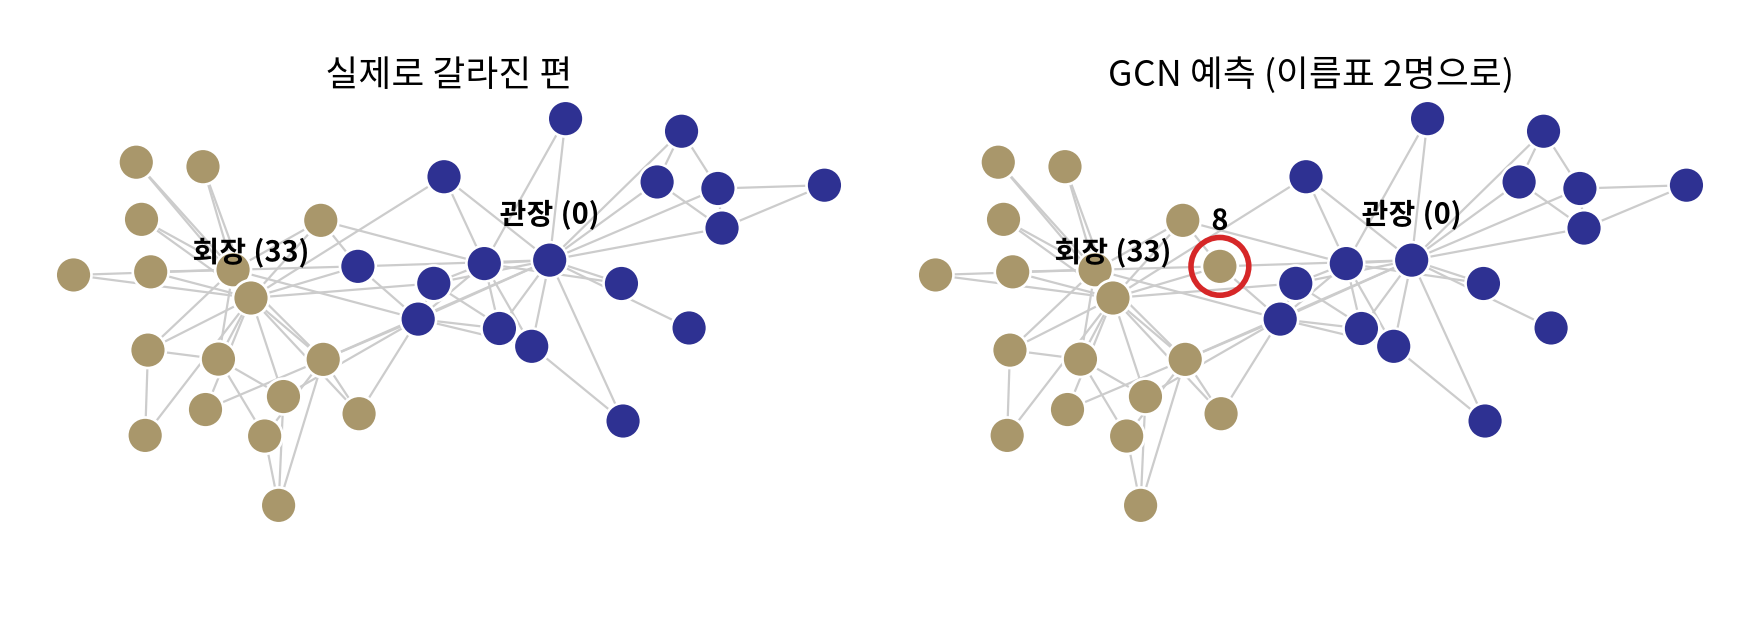
\includegraphics[width=0.84\linewidth]{gc_result.png}\par\vskip0.1em
{\normalsize 특징 = 사람마다 고유 번호 (34칸 원-핫) \quad 은닉 16 \quad 손실은 관장 · 회장 2명에서만}\\[0.2em]
{\large 나머지 32명 중 \kb{31명} 정답 (시드 10개 모두)}\\[0.1em]{\large 틀린 \kq{8번}: 친구 5명 중 3명이 회장 편}
\vfill
\note{실제로 학습해 봤습니다. 특징은 사람마다 고유 번호, 34칸짜리 원-핫 벡터입니다. 사람에 대해 아무것도 모르고 친구 관계만 아는 셈이죠. 2층 GCN, 은닉 16칸으로, 손실은 편을 아는 관장과 회장 두 사람에서만 계산했습니다. 그런데도 나머지 32명 중 31명을 맞혔고, 시드를 10번 바꿔도 모두 31명이었습니다. 틀린 한 명은 8번인데, 친구 다섯 명 중 세 명이 회장 편이었습니다. 친구 관계만 보면 회장 편이라고 하는 게 자연스러운데, 실제로는 관장 편으로 갔습니다.}
\end{frame}

% --- 층 수
\begin{frame}{층은 몇 개가 좋을까}
\vfill
\begin{columns}[c]
\column{0.55\linewidth}\centering
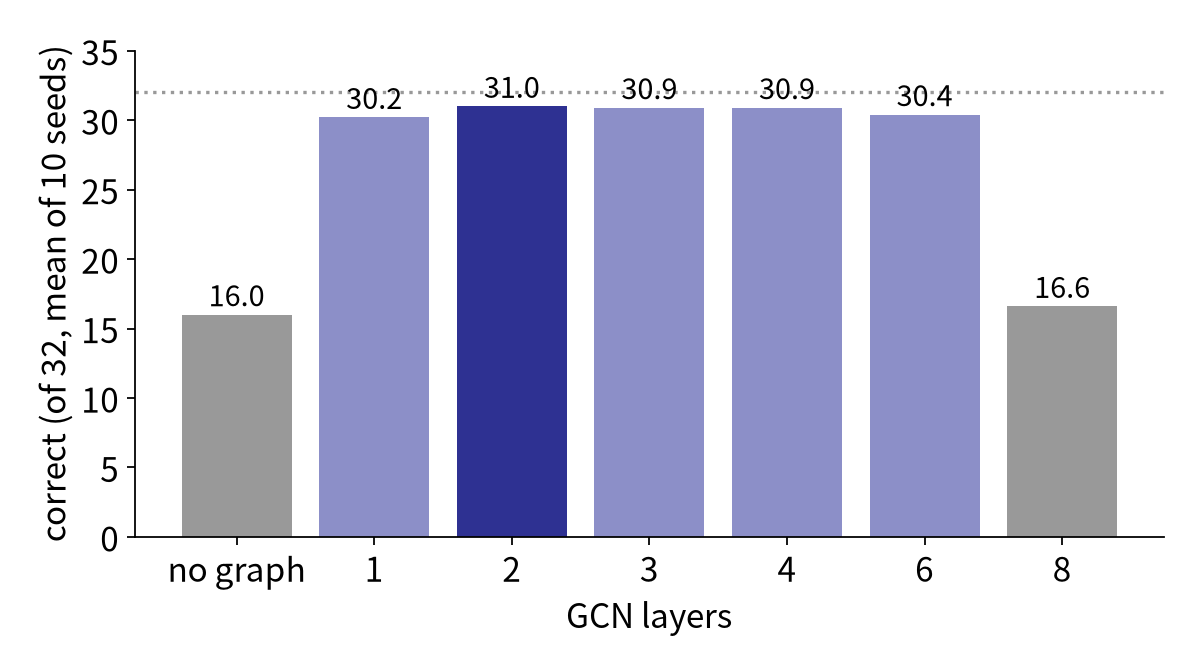
\includegraphics[width=\linewidth]{gc_layers.png}
\column{0.43\linewidth}
{\large 그래프를 안 쓰면 (0층): \kq{16명}}\\
{\small 이름표 없는 사람은 배울 게 없다: 모두 한쪽}\\[0.6em]
{\large 1 $\sim$ 6층: 30 $\sim$ \kb{31명}}\\
{\small 32명 중 29명이 관장 · 회장의 직접 친구}\\[0.6em]
{\large 8층: 다시 \kq{16.6명}}\\
{\small 평균을 너무 많이 내면 모두 비슷해진다 (\textbf{과평활}, over-smoothing)}
\end{columns}
\vfill
\note{층 수를 바꿔 봤습니다. 그래프를 안 쓰고 고유 번호만으로 학습하면 32명 중 16명, 모두 한쪽으로 찍는 것과 같습니다. 이름표 없는 사람의 번호는 학습에 한 번도 쓰이지 않으니까요. 1층부터 6층까지는 30명에서 31명입니다. 이 동아리는 32명 중 29명이 관장이나 회장의 직접 친구라서 1층으로도 꽤 됩니다. 그런데 8층을 쌓으면 다시 16.6명으로 무너집니다. 평균을 여덟 번 내면 모든 사람의 정보가 비슷해져 구분이 안 됩니다. 이걸 과평활, over-smoothing이라 합니다. 그래서 GCN은 보통 2, 3층만 씁니다.}
\end{frame}

% --- 쓰임
\begin{frame}{어디에 쓰나}
\vfill
\centering
\renewcommand{\arraystretch}{1.5}
{\large\begin{tabular}{lll}
논문 분류 & Cora: 논문 2,708편, 이름표 140개 & 정확도 \kb{81.5\%}\\
분자 · 단백질 & 원자 = 노드, 결합 = 엣지 & 기능 예측 (DeepFRI)\\
도로 교통 & 교차로 = 노드, 도로 = 엣지 & 속도 예측 (STGCN)\\
추천 & 사용자 · 상품 = 노드 & 핀터레스트 PinSage
\end{tabular}}\vskip0.8em
{\large 그래프 신경망 (GNN): GCN, GraphSAGE (2017), GAT (2018, 이웃마다 \textbf{어텐션})}
\vfill
\note{GCN은 연결된 데이터에 두루 쓰입니다. 원 논문은 논문 2708편과 인용 5429개로 된 Cora 데이터에서, 이름표 140개만으로 81.5퍼센트를 맞혔습니다. 분자와 단백질에서는 원자가 노드, 결합이 엣지이고, 단백질 기능을 예측하는 DeepFRI가 GCN을 씁니다. 도로 교통에서는 교차로가 노드, 도로가 엣지이고, STGCN이 속도를 예측합니다. 핀터레스트는 사용자와 상품의 그래프로 추천을 합니다. GCN 외에도 이웃을 뽑아 모으는 GraphSAGE, 이웃마다 어텐션으로 비율을 정하는 GAT 같은 그래프 신경망 가족이 있습니다.}
\end{frame}

\section{연습}
% --- 문제풀이
\begin{frame}{문제풀이}
\vfill
\begin{enumerate}
\item 손 계산 그래프에서 B 의 친구가 A 와 D 둘이라면, 1층 뒤 B 의 값은? (평균, 자기 포함)\vskip0.8em
\item 친구 수가 (자기 포함) 4 인 사람과 9 인 사람 사이의 $\hat{A}_{ij}$ 는?\vskip0.8em
\item 노드 34개, 특징 34칸, 은닉 16, 출력 2 인 2층 GCN 의 가중치 수는? (편향 포함)\vskip0.8em
\item 8층에서 정답이 16명 근처로 떨어진 이유를 ``평균'' 으로 설명해 보라.
\end{enumerate}
\vfill
\note{1번 답. 자기 0, A의 1, D의 마이너스 1을 평균 내 0입니다. 2번 답. 1 나누기 루트 36, 6분의 1, 약 0.17입니다. 3번 답. 34 곱하기 16 더하기 16, 560개와 16 곱하기 2 더하기 2, 34개를 더해 594개입니다. 노드 수가 늘어도 W 크기는 특징 칸 수에만 달려 있습니다. 4번 답. 평균을 여러 번 내면 연결된 사람들의 값이 점점 같아져서, 결국 모두 거의 같은 벡터가 되어 두 편을 구분할 수 없습니다.}
\end{frame}

% --- 실습
\begin{frame}{실습}
\vfill
\centering\begin{tabular}{rl}
\large 1 & 손 계산 그래프로 평균 한 층 · 두 층, $\hat{A}$ 만들기\\[0.5em]
\large 2 & 가라테 클럽 2층 GCN 직접 구현 (numpy 식 $\to$ PyTorch) $\to$ 31 / 32\\[0.5em]
\large 3 & 층 수 바꾸기 (과평활), 사람마다 두 점수를 그려 보기
\end{tabular}\vskip1em
Zachary karate club (\texttt{networkx}) \\[0.4em]\href{https://colab.research.google.com/github/SuminHan/book-ml/blob/main/slides/v2/ml1/week13/gcn/lab/gcn.ipynb}{\textcolor{ksagolddk}{▶ Colab에서 실습 노트북 열기}}
\vfill
\note{실습은 세 부분입니다. 첫째, 손 계산 그래프로 평균을 한 층, 두 층 내 보고, GCN의 A 햇을 만듭니다. 둘째, 가라테 클럽에 2층 GCN을 직접 구현해 31명을 맞히는지 확인합니다. 셋째, 층 수를 바꿔 과평활을 보고, 사람마다 두 편의 점수를 평면에 그려 봅니다.}
\end{frame}

\section{정리}
% --- 정리
\begin{frame}{정리}
\vfill
\centering\large\begin{tabular}{l}
그래프 = 노드 + 엣지 (인접 행렬 $A$) \quad 이웃 수가 제각각, 순서 없음\\[0.5em]
\textbf{GCN}: $H' = \sigma(\hat{A} H W)$, \quad $\hat{A} = D^{-1/2}(A + I) D^{-1/2}$ \quad 나와 친구들의 \kb{평균}\\[0.5em]
1층 = 친구, 2층 = 친구의 친구 \quad 모든 노드가 같은 $W$ (그래프 합성곱)\\[0.5em]
가라테: 이름표 2개로 \kb{31 / 32} \quad 8층은 과평활로 16.6
\end{tabular}
\vfill
\note{정리합니다. 그래프는 노드와 엣지이고, 이웃 수가 제각각이며 순서가 없습니다. GCN은 A 햇 H W에 활성화를 씌워, 각 노드의 정보를 나와 친구들의 평균으로 바꿉니다. 1층은 친구, 2층은 친구의 친구까지 보고, 모든 노드가 같은 W를 써서 그래프 합성곱이라 부릅니다. 가라테 동아리에서는 이름표 2개만으로 32명 중 31명을 맞혔고, 8층은 과평활로 무너졌습니다.}
\end{frame}
\end{document}
